% Options for packages loaded elsewhere
\PassOptionsToPackage{unicode}{hyperref}
\PassOptionsToPackage{hyphens}{url}
\PassOptionsToPackage{dvipsnames,svgnames,x11names}{xcolor}
\documentclass[
  10pt,
]{article}
\usepackage{xcolor}
\usepackage[margin=1in]{geometry}
\usepackage{amsmath,amssymb}
\setcounter{secnumdepth}{-\maxdimen} % remove section numbering
\usepackage{iftex}
\ifPDFTeX
  \usepackage[T1]{fontenc}
  \usepackage[utf8]{inputenc}
  \usepackage{textcomp} % provide euro and other symbols
\else % if luatex or xetex
  \usepackage{unicode-math} % this also loads fontspec
  \defaultfontfeatures{Scale=MatchLowercase}
  \defaultfontfeatures[\rmfamily]{Ligatures=TeX,Scale=1}
\fi
\usepackage{lmodern}
\ifPDFTeX\else
  % xetex/luatex font selection
\fi
% Use upquote if available, for straight quotes in verbatim environments
\IfFileExists{upquote.sty}{\usepackage{upquote}}{}
\IfFileExists{microtype.sty}{% use microtype if available
  \usepackage[]{microtype}
  \UseMicrotypeSet[protrusion]{basicmath} % disable protrusion for tt fonts
}{}
\makeatletter
\@ifundefined{KOMAClassName}{% if non-KOMA class
  \IfFileExists{parskip.sty}{%
    \usepackage{parskip}
  }{% else
    \setlength{\parindent}{0pt}
    \setlength{\parskip}{6pt plus 2pt minus 1pt}}
}{% if KOMA class
  \KOMAoptions{parskip=half}}
\makeatother
\usepackage{longtable,booktabs,array}
\usepackage{caption}
\captionsetup[table]{skip=6pt}
\newcounter{none} % for unnumbered tables
\usepackage{calc} % for calculating minipage widths
% Correct order of tables after \paragraph or \subparagraph
\usepackage{etoolbox}
\makeatletter
\patchcmd\longtable{\par}{\if@noskipsec\mbox{}\fi\par}{}{}
\makeatother
% Allow footnotes in longtable head/foot
\IfFileExists{footnotehyper.sty}{\usepackage{footnotehyper}}{\usepackage{footnote}}
\makesavenoteenv{longtable}
\usepackage{graphicx}
\makeatletter
\newsavebox\pandoc@box
\newcommand*\pandocbounded[1]{% scales image to fit in text height/width
  \sbox\pandoc@box{#1}%
  \Gscale@div\@tempa{\textheight}{\dimexpr\ht\pandoc@box+\dp\pandoc@box\relax}%
  \Gscale@div\@tempb{\linewidth}{\wd\pandoc@box}%
  \ifdim\@tempb\p@<\@tempa\p@\let\@tempa\@tempb\fi% select the smaller of both
  \ifdim\@tempa\p@<\p@\scalebox{\@tempa}{\usebox\pandoc@box}%
  \else\usebox{\pandoc@box}%
  \fi%
}
% Set default figure placement to htbp
\def\fps@figure{htbp}
\makeatother
\setlength{\emergencystretch}{3em} % prevent overfull lines
\providecommand{\tightlist}{%
  \setlength{\itemsep}{0pt}\setlength{\parskip}{0pt}}
\usepackage{bookmark}
\IfFileExists{xurl.sty}{\usepackage{xurl}}{} % add URL line breaks if available
\urlstyle{same}
% fallback for those not using the hyperref driver hyperxmp:
\makeatletter
\@ifundefined{xmpquote}{\newcommand{\xmpquote}[1]{#1}}{}
\makeatother
\hypersetup{
  colorlinks=true,
  linkcolor={Maroon},
  filecolor={Maroon},
  citecolor={Blue},
  urlcolor={Blue},
  pdfcreator={LaTeX via pandoc}}

\title{CS683 PA1: Task1}
\author{\textbf{Team: Huffman} \\[3pt]
  Shaik Awez Mehtab (23b1080), Satyam Sinoliya (23b0958), \\
  Gautam Siddarth (23b0957), Mohana Evuri (23b1017)}
\date{}

\begin{document}
\maketitle
\section{Task 1: 2D Convolution}\label{task-1-2d-convolution}

\subsection{Setup}\label{setup}

\begin{itemize}
\tightlist
\item
  Intel Core i5-12450H (4 P-cores + 4 E-cores). L1d 48 KiB/core, L2 1.25
  MiB/P-core, L3 12 MiB shared.
\item
  Hardware prefetchers are \textbf{disabled}.
\item
  Everything pinned with \texttt{taskset\ -c\ 2}, so the process cannot
  migrate between a P-core and an E-core mid-run.
\item
  \texttt{./bin/conv} is the given harness, used for the graded result.
\item
  \texttt{bench/} is a report-only harness that runs exactly one kernel with no
  correctness pass, so \texttt{perf} counters belong to that kernel alone. All
  comparison tables and plots come from it, best-of-7, with stages interleaved.
  It also holds the 128-bit and untiled SIMD versions needed for 1C and 1D; the
  five graded files are untouched by them.
\item
  Absolute times drift by up to 2x with machine temperature, so only
  compare numbers within one table.
\end{itemize}

\subsection{Task 1A: Loop reordering and
unrolling}\label{task-1a-loop-reordering-and-unrolling}

\subsubsection{What is changed}\label{what-is-changed}

\begin{itemize}
\tightlist
\item
  \textbf{Reordering.} The naive version goes over the $W * H$ image only
  once, computing each pixel using the whole kernel. With the reordering
  we go over the whole $W * H$ image $K^2$ times, only adding the effect
  of one kernel element to the output. This requires the output to be
  zeroed first.
\item
  \textbf{Unrolling.} On top of reordering, unrolled the innermost
  \texttt{ox} loop by $k$, checking for different $k$ values, as
  described further. This was done by manually writing $k$ statements for
  computing \texttt{o[ox + 0],...,o[ox + k - 1]} inside the loop.
\end{itemize}

\subsubsection{1. What motivated the
changes?}\label{what-motivated-the-changes}

\begin{itemize}
\tightlist
\item
  The naive version fetches a kernel element for every tap of every
  output pixel. These always hit L1, but each is still a load instruction
  plus its address arithmetic.
\item
  After reordering the weight is constant for a whole pass, so it stays
  in a register and those instructions disappear.
\item
  Unrolling then removes the loop overhead that is left, which is a large
  fraction of the instruction stream when the body is only 4
  instructions.
\end{itemize}

\subsubsection{2. What considerations did I take into
account?}\label{what-considerations-did-i-take-into-account}

\begin{itemize}
\item
  Kept \texttt{ker[ky * K + kx]} for each outer two loop iteration in a
  variable, so this is stored in a register instead. If we instead used it
  directly, the compiler would not necessarily do that (replace that with
  something stored in a register), because it can't detect another pointer with
  same value could've modified the underlying value (eg. out). So it reads
  \texttt{ker} each inner iteration, which we're eliminating.

\item
  \texttt{ox} is the innermost loop, so consecutive iterations touch
  consecutive addresses, which is the best case for the cache.

\item
\textbf{Unroll factor:} As mentioned before, tried various unroll factors, for
which got these as time taken (in ms), for the corresponding params (K=3):

{\def\LTcaptype{none} % do not increment counter
\begin{longtable}[]{@{}lllll@{}}
\toprule\noalign{}
factor & 256 & 512 & 1024 & 2048 \\
\midrule\noalign{}
\endhead
\bottomrule\noalign{}
\endlastfoot
1 & 0.365 & 1.489 & 6.306 & \textasciitilde41 \\
2 & 0.341 & 1.409 & 6.131 & \textasciitilde41 \\
4 & 0.321 & 1.368 & 5.829 & \textasciitilde41 \\
8 & 0.326 & 1.357 & 5.972 & \textasciitilde41 \\
16 & 0.312 & 1.363 & 5.793 & \textasciitilde41 \\
\end{longtable}
}

\begin{itemize}
\tightlist
\item
  Loop overhead is \textasciitilde2 instructions per iteration, so its share
  falls as 1/factor: 33\% at 1, 11\% at 4, 5.5\% at 8. Most of the gain is
  already there by 4, and 4 vs 8 is within noise.
\item
  \texttt{W} is only guaranteed to be a multiple of 8, so 8 is the largest
  factor that divides every legal \texttt{W}. We used 8.
\item
  At 16 the body overruns the row on legal inputs like \texttt{W=8} and
  \texttt{W=24}, and the program segfaults on both. Testing further isn't that
  worthy, as the overhead is anyways 1/factor now.
\end{itemize}
\end{itemize}

\subsubsection{3. How effective are the changes, and by which
metric?}\label{how-effective-are-the-changes-and-by-which-metric}

\begin{itemize}
\tightlist
\item
  The main metric we considered is wall-clock speedup over naive.
\item
  Also counted \textbf{bytes moved past L2}, with \texttt{perf\ stat\ -e\
  l2\_rqsts.miss}. This overestimates DRAM traffic, since some of it is served
  by L3, but L3 misses would underestimate it by more.
\end{itemize}

Speedup over naive:

{\def\LTcaptype{none} % do not increment counter
\begin{longtable}[]{@{}
  >{\raggedright\arraybackslash}p{(\linewidth - 10\tabcolsep) * \real{0.1667}}
  >{\raggedright\arraybackslash}p{(\linewidth - 10\tabcolsep) * \real{0.1667}}
  >{\raggedright\arraybackslash}p{(\linewidth - 10\tabcolsep) * \real{0.1667}}
  >{\raggedright\arraybackslash}p{(\linewidth - 10\tabcolsep) * \real{0.1667}}
  >{\raggedright\arraybackslash}p{(\linewidth - 10\tabcolsep) * \real{0.1667}}
  >{\raggedright\arraybackslash}p{(\linewidth - 10\tabcolsep) * \real{0.1667}}@{}}
\toprule\noalign{}
\begin{minipage}[b]{\linewidth}\raggedright
size
\end{minipage} & \begin{minipage}[b]{\linewidth}\raggedright
working set
\end{minipage} & \begin{minipage}[b]{\linewidth}\raggedright
reorder K=3
\end{minipage} & \begin{minipage}[b]{\linewidth}\raggedright
unroll K=3
\end{minipage} & \begin{minipage}[b]{\linewidth}\raggedright
reorder K=5
\end{minipage} & \begin{minipage}[b]{\linewidth}\raggedright
unroll K=5
\end{minipage} \\
\midrule\noalign{}
\endhead
\bottomrule\noalign{}
\endlastfoot
128 & 128 KiB & 1.26x & 1.46x & 1.30x & 1.50x \\
256 & 0.5 MiB & 1.23x & 1.44x & 1.31x & 1.42x \\
512 & 2 MiB & 1.26x & 1.29x & 1.24x & 1.29x \\
1024 & 8 MiB & 0.99x & 1.03x & 1.09x & 1.13x \\
2048 & 32 MiB & 0.61x & 0.65x & 0.65x & 0.71x \\
\end{longtable}
}

So both changes help up to 512, break even at 1024, and are a clear
\textbf{loss} at 2048.

\textbf{Small sizes:} Everything fits in cache, so nothing is waiting on
memory and the loop is limited by instruction count. Measured with
\texttt{perf} at 256x256:

\begin{longtable}[]{@{}llll@{}}
\toprule\noalign{}
version & instructions/pixel (rough) & IPC & cycles/pixel (rough) \\
\midrule\noalign{}
\endhead
\bottomrule\noalign{}
\endlastfoot
naive & 100.6 & 4.76 & 21.2 \\
reorder & 64.0 & 3.80 & 16.8 \\
unroll & 41.5 & 2.57 & 16.1 \\
\end{longtable}

\begin{itemize}
\tightlist
\item
  Naive runs at IPC 4.76, close to the core's maximum of about 6
  instructions per cycle, so it isn't waiting on anything, it's just
  executing too many instructions.
\item
  Reordering cuts instructions per pixel by 36\% and unrolling by a
  further 35\%.
\item
  For reordering that's the fewer loads, since we pre-store
  \texttt{ker[...]}. For unrolling it's the fewer loop update and check
  instructions.
\item
  IPC also drops (4.76 to 3.80), since removing independent loads removes
  some parallelism, but instructions fall faster, so cycles/pixel still
  reduces.
\end{itemize}

\textbf{Large sizes regress} because reordering trades instruction count
for memory traffic. The $K^2$ passes each re-read the input and do a
read-modify-write of the output, so the traffic should be about
$K^2 = 9$ times the compulsory minimum. Measured at 2048x2048, K=3,
against a compulsory 32 MiB (16 MiB in read once, 16 MiB out written
once):

{\def\LTcaptype{none} % do not increment counter
\begin{longtable}[]{@{}lllll@{}}
\toprule\noalign{}
version & L2 traffic & vs compulsory & time & effective rate \\
\midrule\noalign{}
\endhead
\bottomrule\noalign{}
\endlastfoot
naive & 40.7 MiB & 1.27x & 17.4 ms & 2.5 GB/s \\
reorder & 301.6 MiB & 9.43x & 28.4 ms & 11.1 GB/s \\
unroll & 301.6 MiB & 9.42x & 26.7 ms & 11.9 GB/s \\
\end{longtable}
}

\begin{itemize}
\tightlist
\item
  The measured 9.43x matches the predicted 9 passes.
\item
  Naive's 2.5 GB/s is nowhere near any memory limit, so it was never
  memory-bound to begin with, only instruction-bound.
\item
  Reordering fixes the instruction count and immediately runs into the memory
  system instead.
\item
  Whether the 9x traffic actually costs time depends on which cache level
  serves it. Up to 512 it is served by L2/L3 and is nearly free, so the
  instruction saving dominates. At 1024 (8 MiB) it is served by L3 and roughly
  cancels the win. At 2048 (32 MiB) it must come from DRAM and hence the loop
  inverts to 0.61x.
\item
  \textbf{Unroll vs reorder at 2048} differ by only 3\%. \texttt{perf} shows:
  going from unroll factor 4 to 8 removes 3.2\% of instructions (5.997e9 to
  5.808e9) but leaves cycles unchanged (1.6968e9 to 1.6925e9), this is because
  the core is waiting on memory.
\item
  The same unrolling is worth 10-16\% at 256 and 512, where instructions are
  the bottleneck.
\end{itemize}

\textbf{Conclusion.} Both changes are right for the instruction count and
wrong for the memory system once the working set leaves cache. So we don't
want to undo them, we want the $K^2$ passes to hit cache instead, which is
what tiling does next.

\subsection{Task 1B: Tiling}\label{task-1b-tiling}

\subsubsection{1. Profiling the baseline}\label{profiling-the-baseline}

\begin{itemize}
\tightlist
\item
  L1-D cache size on this machine: \textbf{48 KiB per core}
  (\texttt{lscpu} reports 320 KiB over 8 instances; the 4 P-cores have 48
  KiB each).
\item
  Baseline naive L1-D MPKI, from
  \texttt{perf\ stat\ -e\ instructions,L1-dcache-load-misses} (median of
  3 runs):
\end{itemize}

{\def\LTcaptype{none} % do not increment counter
\begin{longtable}[]{@{}lllll@{}}
\toprule\noalign{}
naive L1-D MPKI & 256 & 512 & 1024 & 2048 \\
\midrule\noalign{}
\endhead
\bottomrule\noalign{}
\endlastfoot
K=3 & 0.95 & 0.38 & 0.20 & 0.12 \\
K=5 & 0.47 & 0.18 & 0.10 & 0.07 \\
K=7 & 0.29 & 0.12 & 0.06 & 0.04 \\
K=9 & 0.20 & 0.10 & 0.06 & 0.05 \\
\end{longtable}
}

\begin{itemize}
\tightlist
\item
  MPKI falls with K only because instructions per pixel grows as $K^2$
  (104, 218, 380, 590 for K=3,5,7,9) while the miss count barely moves.
  K does not change the picture; the rest of 1B uses K=3.
\end{itemize}

\subsubsection{2. Tiled implementation}\label{tiled-implementation}

\begin{itemize}
\tightlist
\item
  \texttt{conv\_tile.cpp} processes the output in $TH * TW$ blocks. For
  each block it zeroes the block, then runs the $K^2$ passes over that
  block alone.
\item
  The block and its corresponding $(TH+K-1) * (TW+K-1)$ input block stay in
  cache for the whole sweep, instead of being re-fetched $K^2$ times from DRAM.
\end{itemize}

Tile sizes swept at $2048*2048$, \texttt{K=3}. Footprint is output tile + input
block size:

{\def\LTcaptype{none} % do not increment counter
\begin{longtable}[]{@{}lllll@{}}
\toprule\noalign{}
tile & footprint & time (ms) & L1-D MPKI & L2 traffic \\
\midrule\noalign{}
\endhead
\bottomrule\noalign{}
\endlastfoot
16x64 & 8.6 KiB & 13.28 & 16.73 & 40.8 MiB \\
32x128 & 33.3 KiB & 14.06 & 17.25 & 41.9 MiB \\
64x64 & 33.0 KiB & 14.68 & 18.23 & 43.8 MiB \\
64x128 & 65.5 KiB & 13.82 & 17.21 & 45.2 MiB \\
\textbf{64x256} & \textbf{130.5 KiB} & \textbf{13.42} & \textbf{16.72} &
\textbf{44.7 MiB} \\
128x256 & 259.0 KiB & 15.30 & 16.90 & 87.1 MiB \\
128x512 & 517.0 KiB & 15.25 & 16.62 & 113.9 MiB \\
256x512 & 1030.0 KiB & 16.35 & 16.70 & 253.6 MiB \\
\end{longtable}
}

I kept \textbf{64x256}. 16x64 is 1\% faster at 2048 but slower at 1024
(2.999 vs 2.819 ms), so 64x256 is the better all-round choice.

\begin{figure}
\centering
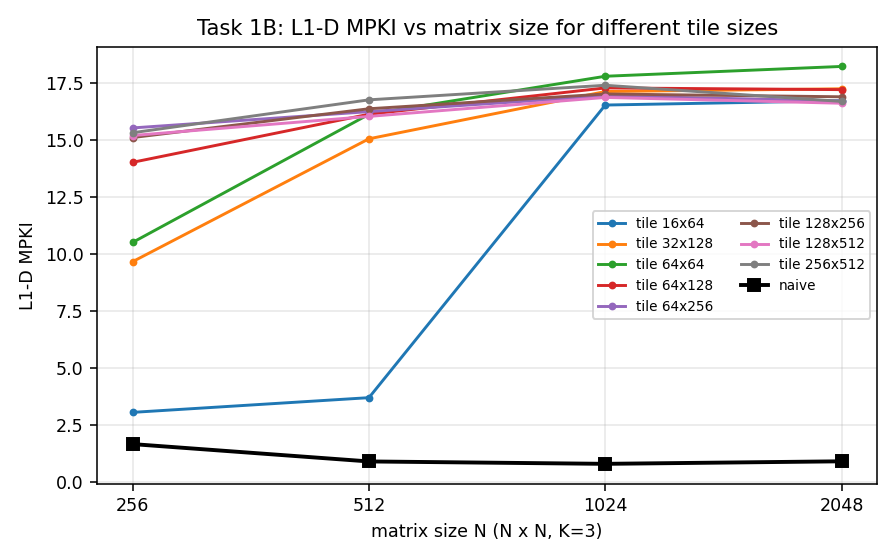
\includegraphics[width=0.88\linewidth,height=\textheight,keepaspectratio,alt={L1-D MPKI vs matrix size for different tile sizes. Every tiled curve sits far above naive, because tiling targets L2 rather than L1.}]{../plots/task1b_mpki_vs_size.png}
\caption{L1-D MPKI vs matrix size for different tile sizes. Every tiled
curve sits far above naive, because tiling targets L2 rather than L1.}
\end{figure}

\begin{figure}
\centering
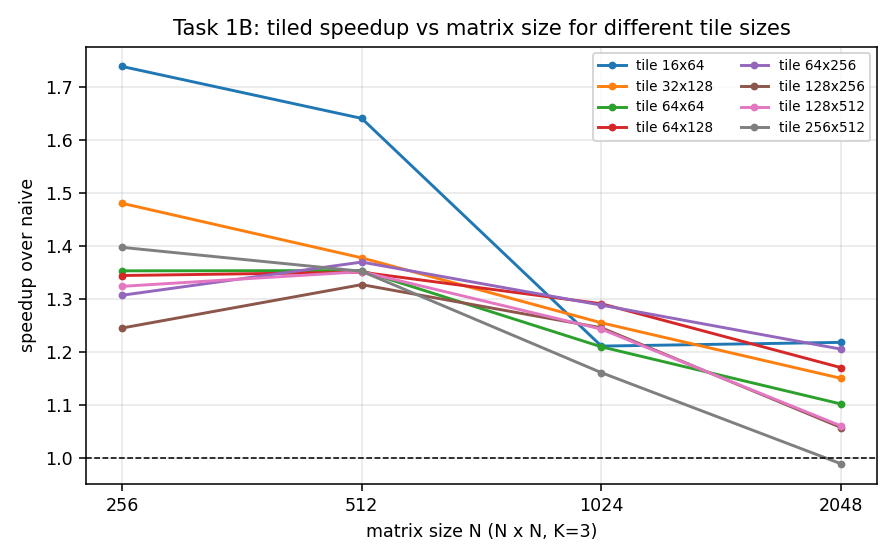
\includegraphics[width=0.88\linewidth,height=\textheight,keepaspectratio,alt={Tiled speedup vs matrix size for different tile sizes.}]{../plots/task1b_speedup_vs_size.png}
\caption{Tiled speedup vs matrix size for different tile sizes.}
\end{figure}

\begin{figure}
\centering
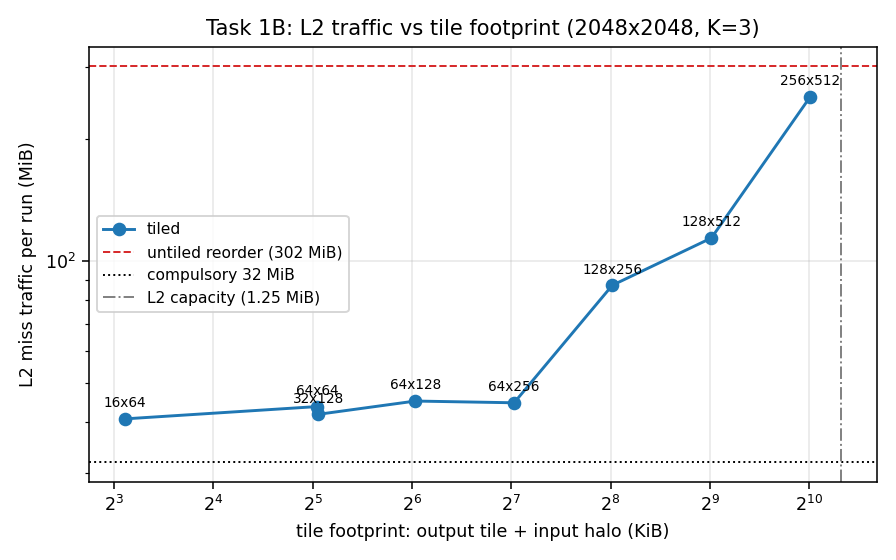
\includegraphics[width=0.88\linewidth,height=\textheight,keepaspectratio,alt={L2 traffic vs tile footprint at $2048*2048$. Traffic sits at the compulsory floor while the footprint stays well below L2 capacity, then climbs towards the untiled figure.}]{../plots/task1b_l2_vs_tile.png}
\caption{L2 traffic vs tile footprint at $2048*2048$. Traffic sits at the
compulsory floor while the footprint stays well below L2 capacity, then
climbs towards the untiled figure.}
\end{figure}

\subsubsection{3. Analysis}\label{analysis}

\textbf{Q1. Change in L1-D MPKI from naive to tiled.}

\begin{itemize}
\tightlist
\item
  It goes \textbf{up}, from 0.12 to 16.8 at $2048*2048$, which looks wrong
  at first.
\item
  MPKI is misses divided by instructions, and tiling changes both.
  Tiling is applied on top of the reordered loop, which already executes
  half as many instructions as naive (49 vs 104 per output pixel), so the
  denominator shrinks.
\item
  The numerator grows too: naive re-reads its 3 active rows straight out
  of L1, whereas the tiled loop streams a 130 KiB tile that does not fit
  in a 48 KiB L1, so its reuse is served by \textbf{L2, not L1}.
\end{itemize}

The right comparison is tiled against the untiled reordered loop it
replaces, and at the level tiling actually targets (i.e L2):

{\def\LTcaptype{none} % do not increment counter
\begin{longtable}[]{@{}llll@{}}
\toprule\noalign{}
version & L2 traffic & vs compulsory & speedup vs naive \\
\midrule\noalign{}
\endhead
\bottomrule\noalign{}
\endlastfoot
reorder (untiled) & 301.6 MiB & 9.43x & 0.61x \\
tile & 44.9 MiB & 1.40x & 1.17x \\
\end{longtable}
}

Tiling cuts traffic past L2 by \textbf{6.7x}, from 9.4 passes over the
image down to 1.4, which is what we wanted. It was never about L1 MPKI.

\textbf{Q2. How MPKI varies with matrix size and tile size.}

\begin{itemize}
\tightlist
\item
  Fixing the size at 2048 and varying the tile, MPKI barely moves, it stays
  at 16.6-18.2. Every tile we tried is either bigger than the 48 KiB L1 or
  just streams through it, so none of them change what L1 sees.

\item
  Varying the matrix size, the only tile that behaves differently is 16x64,
  whose 8.6 KiB footprint actually fits in L1: MPKI is 3.06 at 256 and 3.71
  at 512, against 15-17 for every bigger tile.

\item
  Even 16x64 goes back up to \textasciitilde16.5 past 1024. The padded row
  stride is 2050 floats there, so the 18 halo rows it touches are
  \textasciitilde8.2 KiB apart, and they start conflicting in a 12-way L1.

\item
  L2 is where the working set argument actually shows up. Traffic sits at
  the \textasciitilde41-45 MiB floor while the footprint is under
  \textasciitilde130 KiB, then climbs: 87 MiB at 259 KiB, 114 MiB at 517
  KiB, 254 MiB at 1030 KiB, which is almost the untiled 302 MiB.

\item
  So the tile should be sized well \textbf{below} L2, not at it. At 80\% of
  the 1.25 MiB L2 we've lost nearly all the benefit, because the tile has to
  survive $K^2$ passes while the streaming input is competing for the same
  cache.
\end{itemize}

\textbf{Q3. Did I achieve a speedup?}

Yes, and how it changes with size matters:

{\def\LTcaptype{none} % do not increment counter
\begin{longtable}[]{@{}llllll@{}}
\toprule\noalign{}
size & 128 & 256 & 512 & 1024 & 2048 \\
\midrule\noalign{}
\endhead
\bottomrule\noalign{}
\endlastfoot
tile vs naive (K=3) & 1.38x & 1.40x & 1.22x & 1.18x & 1.17x \\
tile vs naive (K=5) & 1.42x & 1.28x & 1.34x & 1.30x & 1.33x \\
tile vs reorder (K=3) & 1.10x & 1.14x & 0.97x & 1.19x & 1.91x \\
\end{longtable}
}

\begin{itemize}
\tightlist
\item
  Against naive the gain is modest, but against the reordered loop it is 1.91x
  at 2048, turning a 0.61x regression into a 1.17x speedup.
\item
  What's left is that this stage is still scalar: 49 instructions per output
  pixel, and 2 loads + 1 store + 1 FMA for every single element. No amount of
  cache tuning fixes that, SIMD does.
\end{itemize}

\subsection{Task 1C: SIMD}\label{task-1c-simd}

\subsubsection{1. Baseline instruction
count}\label{baseline-instruction-count}

Naive at 2048x2048, K=3: \textbf{0.436e9 instructions per run}, about 104 per
output pixel.

\subsubsection{2. Implementation}\label{implementation}

\begin{itemize}
\tightlist
\item
  \texttt{conv\_simd.cpp} keeps the tiled nesting and replaces the scalar inner
  loop with 256-bit AVX2.
\item
  \texttt{bench/conv\_simd128.cpp} is the same code at 128-bit, for the
  width comparison.
\item
  \textbf{AVX-512 is not available on this CPU}, so only 128-bit and 256-bit
  are reported.
\end{itemize}

\subsubsection{3. Instruction count and
performance}\label{instruction-count-and-performance}

Per run at 2048x2048, K=3:

{\def\LTcaptype{none} % do not increment counter
\begin{longtable}[]{@{}lllll@{}}
\toprule\noalign{}
version & instructions & per output pixel & vs naive & speedup \\
\midrule\noalign{}
\endhead
\bottomrule\noalign{}
\endlastfoot
naive & 0.436e9 & 103.9 & 1.00x & 1.00x \\
tile (scalar) & 0.207e9 & 49.4 & 2.10x fewer & 1.17x \\
simd 128-bit & 0.104e9 & 24.7 & 4.21x fewer & 3.06x \\
simd 256-bit & 0.080e9 & 19.0 & 5.48x fewer & 3.82x \\
\end{longtable}
}

\begin{itemize}
\tightlist
\item
  Going from naive to 256-bit SIMD, instructions drop \textbf{5.48x}. One
  \texttt{vfmadd} now does 8 elements where the scalar loop needed one
  multiply-add each, and the loop runs 8 times fewer iterations, so the
  loads, stores, increments and branches divide by 8 too.

\item
  We don't get the full 8x because the zeroing pass, the tile bookkeeping
  and the loop setup are the same as before, they don't vectorise.

\item
  Halving the width to 128-bit costs us 1.30x more instructions and 1.25x
  more time, which track each other closely. So we're still mostly limited
  by how many instructions we execute, and doubling the width buys us
  almost the full 2x.
\end{itemize}

\subsubsection{4. Multi-size results}\label{multi-size-results}

Speedup over naive, K=3:

{\def\LTcaptype{none} % do not increment counter
\begin{longtable}[]{@{}llllll@{}}
\toprule\noalign{}
size & 128 & 256 & 512 & 1024 & 2048 \\
\midrule\noalign{}
\endhead
\bottomrule\noalign{}
\endlastfoot
128-bit & 4.09x & 4.01x & 3.72x & 3.17x & 3.06x \\
256-bit & 5.39x & 5.27x & 4.65x & 4.38x & 3.82x \\
\end{longtable}
}

Both widths lose ground as the matrix grows, and 256-bit loses more, so
the gap narrows from 1.32x at N=128 to 1.25x at N=2048. Every size up to
1024 still fits in the 12 MiB L3, but at 2048 the input and output are 32
MiB together, so we're waiting on DRAM. Removing more instructions doesn't
help then, and the wider version reaches that point first.

\begin{figure}
\centering
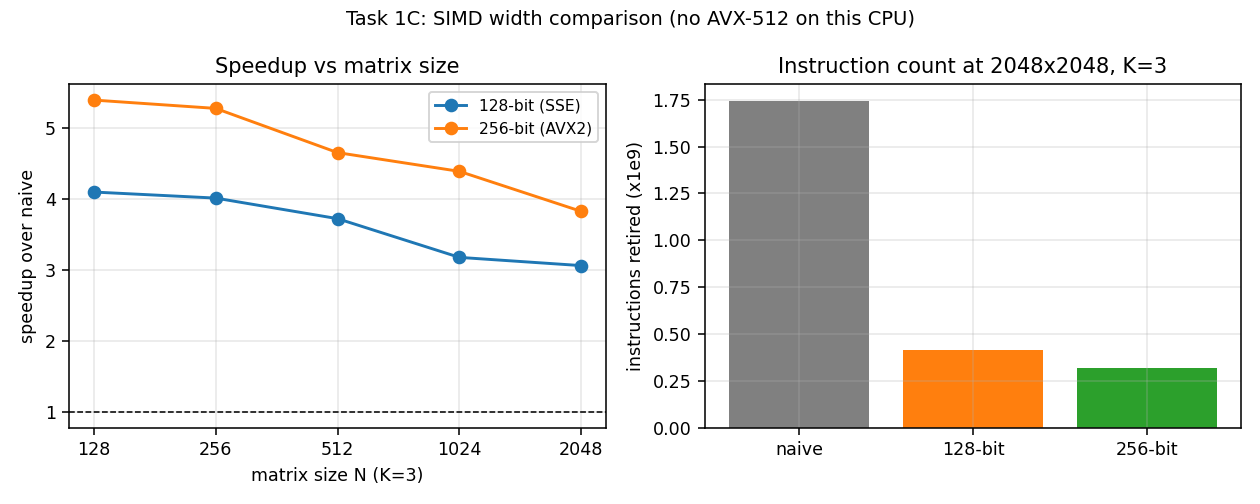
\includegraphics[width=0.98\linewidth,height=\textheight,keepaspectratio,alt={SIMD width comparison: speedup vs matrix size, and instruction count at 2048x2048.}]{../plots/task1c_simd_width.png}
\caption{SIMD width comparison: speedup vs matrix size, and instruction
count at 2048x2048.}
\end{figure}

\subsubsection{5. Which intrinsics, and
why}\label{which-intrinsics-and-why}

{\def\LTcaptype{none} % do not increment counter
\begin{longtable}[]{@{}
  >{\raggedright\arraybackslash}p{(\linewidth - 2\tabcolsep) * \real{0.5000}}
  >{\raggedright\arraybackslash}p{(\linewidth - 2\tabcolsep) * \real{0.5000}}@{}}
\toprule\noalign{}
\begin{minipage}[b]{\linewidth}\raggedright
intrinsic
\end{minipage} & \begin{minipage}[b]{\linewidth}\raggedright
why
\end{minipage} \\
\midrule\noalign{}
\endhead
\bottomrule\noalign{}
\endlastfoot
\texttt{\_mm256\_fmadd\_ps} & one instruction for multiply-add, half the
uops of separate mul+add and a single rounding step \\
\texttt{\_mm256\_set1\_ps} & broadcasts the kernel weight once per
(ky,kx) pass, so the FMA operand is already in a register \\
\texttt{\_mm256\_load\_ps} / \texttt{\_mm256\_store\_ps} & aligned
access on \texttt{out}. \texttt{alloc\_floats} uses
\texttt{\_mm\_malloc(...,\ 64)} and \texttt{W\ \%\ 8\ ==\ 0}, so every
output row start is 32-byte aligned \\
\texttt{\_mm256\_loadu\_ps} & unaligned load for \texttt{in}. The padded
stride \texttt{W+2p} and the \texttt{+kx} shift both break alignment, so
the aligned form would fault \\
\texttt{\_mm256\_setzero\_ps} & vector zeroing of the output tile \\
\end{longtable}
}

The inner loop computes \textbf{two vectors per iteration}, so 16 columns
instead of 8. This is the same unrolling as in 1A, just on the vector loop.

\begin{itemize}
\tightlist
\item
  We wrote the one-vector version too and measured both. The difference is
  within run-to-run noise: one vector is about 7\% slower at 256, and 3-9\%
  faster at 1024 and 2048.
\item
  So doing two at a time isn't where the speedup comes from. Even with one,
  consecutive iterations write to different addresses, so the CPU already
  overlaps them on its own. We kept two only because it halves the loop
  bookkeeping per element.
\end{itemize}

\subsection{Task 1D: Sabka saath sabka
vikaas}\label{task-1d-sabka-saath-sabka-vikaas}

\texttt{conv\_optimized.cpp} combines everything, and adds a few things the
earlier stages don't have:

\begin{itemize}
\tightlist
\item
  \textbf{Kernel loops innermost.} We accumulate the $K^2$ taps in vector
  registers and write each output vector once, so the read-modify-write of
  \texttt{out} is gone.

\item
  \textbf{Non-temporal stores} (\texttt{\_mm256\_stream\_ps}, with
  \texttt{\_mm\_sfence}), so we never fetch an output line before
  overwriting it.

\item
  \textbf{Software prefetch} (\texttt{\_mm\_prefetch}) on the one input row
  that's actually new, two lines ahead.

\item
  A K=3 version with all 9 weights sitting in registers.
\end{itemize}

\subsubsection{Do the techniques
compose?}\label{do-the-techniques-compose}

At 2048x2048, K=3, each technique measured alone and together:

{\def\LTcaptype{none} % do not increment counter
\begin{longtable}[]{@{}ll@{}}
\toprule\noalign{}
version & speedup \\
\midrule\noalign{}
\endhead
\bottomrule\noalign{}
\endlastfoot
tiling alone (scalar) & 1.17x \\
SIMD alone (untiled) & 1.17x \\
tiling + SIMD & 3.82x \\
all combined & 17.04x \\
\end{longtable}
}

\begin{itemize}
\tightlist
\item
  Separately they give 1.17x each. Adding them would be \textasciitilde1.34x
  and multiplying \textasciitilde1.37x, but together we get \textbf{3.82x},
  which is much more than either.

\item
  That's because each one was hiding the other's benefit. Untiled SIMD gets
  instructions per pixel from 104 down to 18, but at 2048 it moves 9.86x the
  compulsory traffic, so it just waits on DRAM and the extra throughput has
  nowhere to go: 1.17x.

\item
  Tiling gets traffic down to 1.40x compulsory, but the loop is still
  scalar: also 1.17x.

\item
  With both, we're neither waiting on DRAM nor executing too many
  instructions, so the gains that were being masked finally show up.
\end{itemize}

The full version goes further still, and the traffic table shows why:

{\def\LTcaptype{none} % do not increment counter
\begin{longtable}[]{@{}llll@{}}
\toprule\noalign{}
version & L2 traffic & vs compulsory & effective rate \\
\midrule\noalign{}
\endhead
\bottomrule\noalign{}
\endlastfoot
naive & 40.7 MiB & 1.27x & 2.5 GB/s \\
reorder & 301.6 MiB & 9.43x & 11.1 GB/s \\
tile & 44.9 MiB & 1.40x & 3.2 GB/s \\
simd (untiled) & 315.7 MiB & 9.86x & 22.3 GB/s \\
simd (tiled) & 44.0 MiB & 1.38x & 10.2 GB/s \\
optimized & 28.8 MiB & 0.90x & 29.7 GB/s \\
\end{longtable}
}

\begin{itemize}
\tightlist
\item
  \texttt{optimized} moves \textbf{less than the compulsory 32 MiB}. The
  non-temporal stores keep the 16 MiB of output out of the cache entirely,
  so we never read a line just to overwrite it.

\item
  It sustains 29.7 GB/s where the others sit near 10. That's the software
  prefetch doing what the disabled hardware prefetchers would have: starting
  the line fills early enough that misses overlap, instead of happening one
  after another.
\end{itemize}

\subsubsection{Final results}\label{final-results}

Speedup over naive, K=3:

{\def\LTcaptype{none} % do not increment counter
\begin{longtable}[]{@{}llllll@{}}
\toprule\noalign{}
technique & 128 & 256 & 512 & 1024 & 2048 \\
\midrule\noalign{}
\endhead
\bottomrule\noalign{}
\endlastfoot
loop reordering & 1.26x & 1.23x & 1.26x & 0.99x & 0.61x \\
loop unrolling & 1.46x & 1.44x & 1.29x & 1.03x & 0.65x \\
tiling & 1.38x & 1.40x & 1.22x & 1.18x & 1.17x \\
SIMD (AVX2) & 4.72x & 5.42x & 2.23x & 1.60x & 1.17x \\
tiling + SIMD & 5.39x & 5.27x & 4.65x & 4.38x & 3.82x \\
all combined & 18.06x & 17.86x & 19.63x & 19.44x & 17.04x \\
\end{longtable}
}

\begin{figure}
\centering
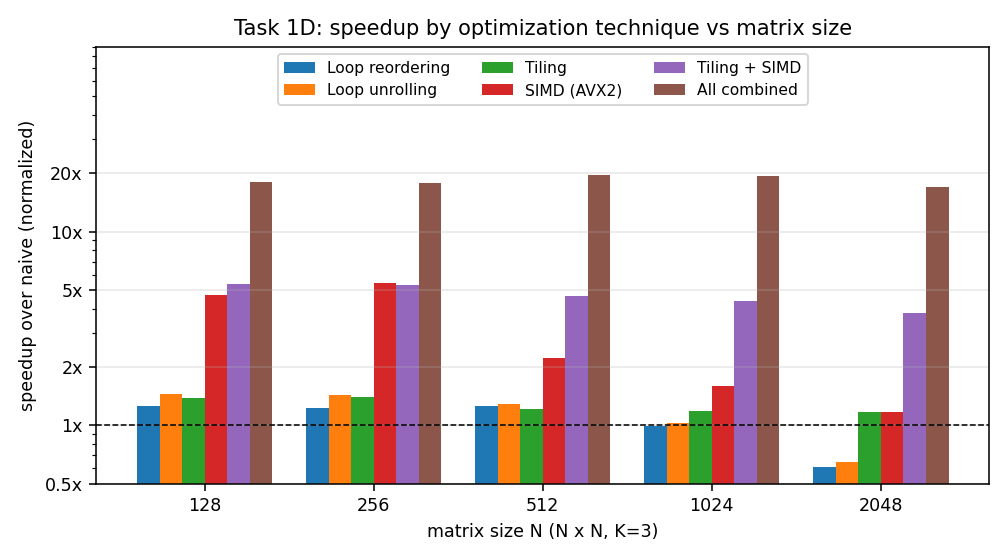
\includegraphics[width=0.98\linewidth,height=\textheight,keepaspectratio,alt={Speedup by optimization technique vs matrix size, grouped bars, log scale.}]{../plots/task1_speedup_vs_size.png}
\caption{Speedup by optimization technique vs matrix size. Log y axis,
since the techniques span 0.61x to 19.6x.}
\end{figure}

The same data as lines, which shows the trend with size more clearly:

\begin{figure}
\centering
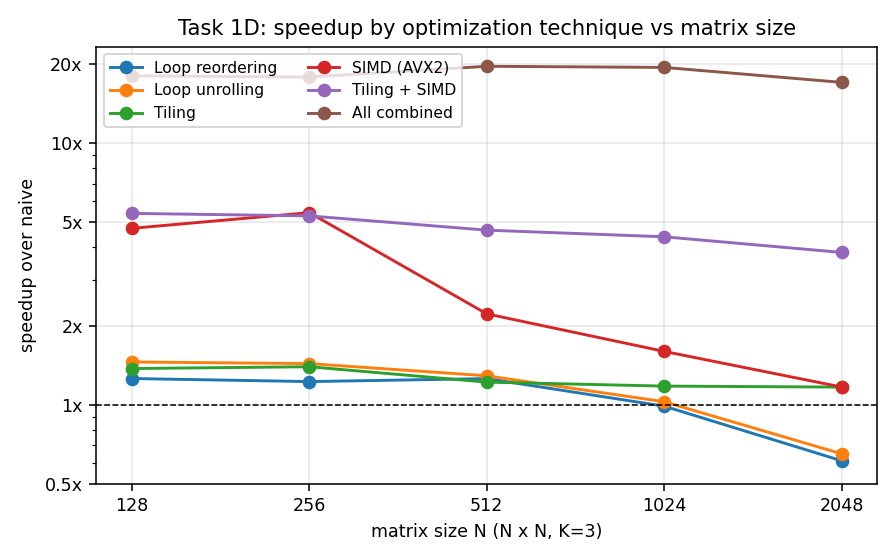
\includegraphics[width=0.88\linewidth,height=\textheight,keepaspectratio,alt={Speedup by optimization technique vs matrix size, line plot, log scale.}]{../plots/task1d_speedup_lines.png}
\caption{Speedup by optimization technique vs matrix size (log scale).}
\end{figure}

Varying kernel size at N=1024:

{\def\LTcaptype{none} % do not increment counter
\begin{longtable}[]{@{}lllll@{}}
\toprule\noalign{}
technique & K=3 & K=5 & K=7 & K=9 \\
\midrule\noalign{}
\endhead
\bottomrule\noalign{}
\endlastfoot
loop reordering & 0.99x & 1.09x & 0.91x & 1.07x \\
loop unrolling & 1.03x & 1.13x & 0.93x & 1.05x \\
tiling & 1.18x & 1.30x & 1.10x & 1.32x \\
SIMD (AVX2) & 1.60x & 1.88x & 1.51x & 1.76x \\
tiling + SIMD & 4.38x & 5.60x & 4.29x & 4.83x \\
all combined & 19.44x & 19.87x & 15.54x & 16.28x \\
\end{longtable}
}

\begin{itemize}
\tightlist
\item
  The scalar stages stay within 0.9-1.3x at every K, so kernel size doesn't
  really matter to them. What they remove scales with $K^2$ just like the
  total work does.

\item
  The vector stages gain a lot more.

\item
  The combined one dips at K=7 and K=9, where we fall back to the generic
  \texttt{convK} and the weights no longer all stay in registers.
\end{itemize}

\begin{figure}
\centering
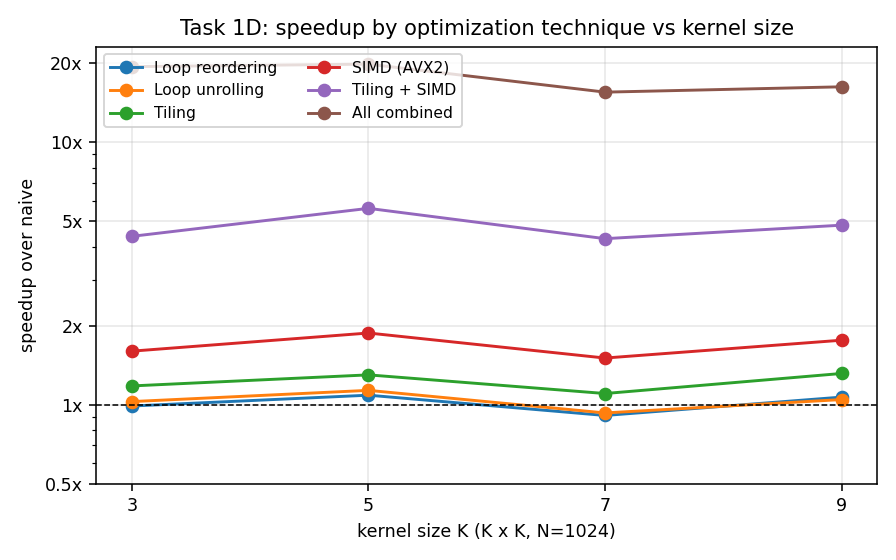
\includegraphics[width=0.88\linewidth,height=\textheight,keepaspectratio,alt={Speedup by optimization technique vs kernel size (log scale).}]{../plots/task1_speedup_vs_kernel.png}
\caption{Speedup by optimization technique vs kernel size (log scale).}
\end{figure}

Graded harness result (\texttt{./bin/conv}, H=W=2048, K=3, seed 1234):

\begin{verbatim}
correctness : 40 / 40   (5 of 5 stages correct)
optimized   : 13.38x  ->  60 / 60  speedup points
TOTAL       : 100 / 100
\end{verbatim}

\begin{itemize}
\tightlist
\item
  The speedup swings between \textasciitilde12x and 22x run to run, with
  machine temperature and with whatever the previous stage left in the
  caches. The top tier needs 8x, so we get 100 / 100 every time.

\item
  We also checked all five stages against naive at W=8, W=24, 333x64,
  512x512, 1000x1024 and 2048x2048, for K=3,5,7. The largest difference is
  \textasciitilde2e-6, which is just float rounding from adding in a
  different order.
\end{itemize}

\end{document}
